\documentclass[a4paper,12pt]{article}

% --- بسته‌های مورد نیاز ---
\usepackage{fontspec}
\usepackage{graphicx}
\usepackage{caption}
\usepackage{float}
\usepackage{amsmath, amssymb}
\usepackage{xepersian}
\usepackage{xcolor}
\usepackage{listings}
\usepackage{courier} % فونت کدها

% --- تعریف رنگ‌ها ---
\definecolor{gray}{rgb}{0.5,0.5,0.5}
\definecolor{orange}{rgb}{1,0.5,0}
\definecolor{codegray}{rgb}{0.95,0.95,0.95}

% --- تنظیم فونت فارسی ---
\settextfont{Vazirmatn Medium}

% --- تنظیمات لیست‌کد (lstlisting) ---
\lstset{
	backgroundcolor=\color{codegray},
	basicstyle=\ttfamily\normalsize,
	keywordstyle=\color{blue}\bfseries,
	commentstyle=\color{gray}\itshape,
	stringstyle=\color{orange},
	numbers=left,
	numberstyle=\tiny\color{gray},
	stepnumber=1,
	numbersep=8pt, % فاصله شماره خطوط از کد
	xleftmargin=15pt,
	frame=single,
	breaklines=true,
	breakatwhitespace=true,
	tabsize=2,
	showspaces=false,
	showstringspaces=false,
	showtabs=false,
	captionpos=b,
	language=C
}

% --- بارگذاری آخر xepersian ---
\begin{document}
	
	\thispagestyle{empty}  % ← این خط شماره صفحه‌ی صفحه اول رو حذف می‌کنه
	
	\begin{center}
		{\Huge \textbf{بسم‌الله‌الرحمن‌الرحیم}}\\[2cm] % فاصله پایین

		{\LARGE \textbf{درخت های قرمز-سیاه - Red-Black Trees}}\\[1cm] % عنوان

		{\large \ مرداد 1404}
	\end{center}
	
		\vspace{500pt}
	% --- اطلاعات سند ---

	\tableofcontents
	\newpage
	
	\section{مقدمه}
	
	Red-black  و یا درخت های قرمز و سیاه درخت های جستجوی دودویی هستند که هر گره آنها دارای رنگ قرمز و یا مشکی است. درخت red-black دارای ارتفاع   \lr{log n} است ، بنابراین عملیات‌های درج، جستجو و حذف در آن در بدترین حالت \lr{O(log n)}  زمان می‌برند.
	
	
	\section{تعریف درخت قرمز-سیاه}
	درخت قرمز-سیاه نوعی \lr{Binary Search Tree} است که در آن به هر گره یک رنگ (قرمز یا سیاه) نسبت داده می‌شود. قوانین رنگ‌بندی و چرخش‌ها باعث حفظ توازن درخت در حین عملیات درج و حذف می‌شوند.
	
	\begin{figure}[H]
		\centering
		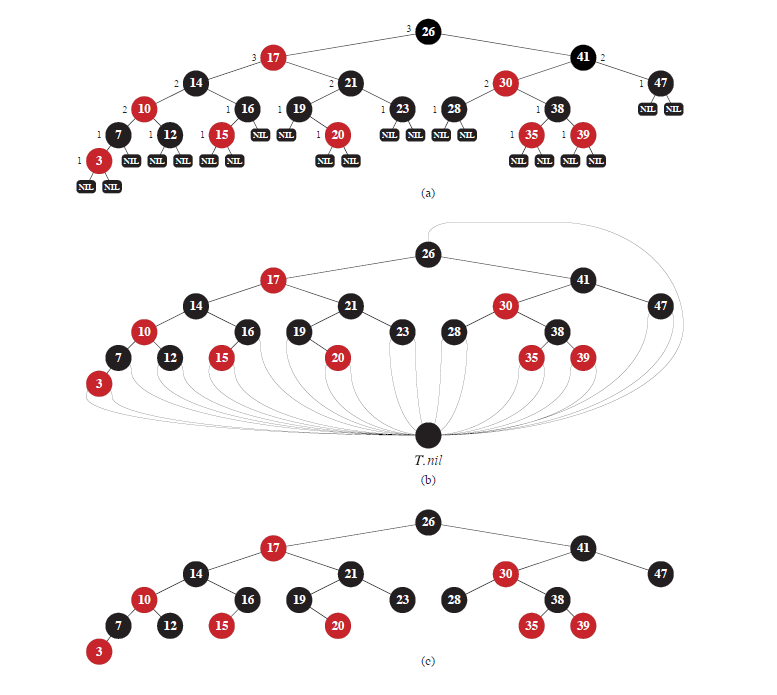
\includegraphics[width=1\textwidth]{img/definition-example.png} % کاربر باید این تصویر را فراهم کند
		\caption{نمونه تصویر درخت سیاه-قرمز x}
	\end{figure}
	
	\section{ویژگی‌های درخت قرمز-سیاه}
	\begin{enumerate}
		\item هر گره یا قرمز است یا سیاه.
		\item ریشه همیشه سیاه است.
		\item همه‌ی برگ‌ها (گره‌های NIL یا تهی) سیاه هستند.
		\item اگر گره‌ای قرمز باشد، فرزندان آن حتماً سیاه هستند.
		\item تعداد گره‌های سیاه در هر مسیر از یک گره تا برگ‌هایش باید یکسان باشد.
	\end{enumerate}
	
	
	\begin{figure}[H]
		\centering
		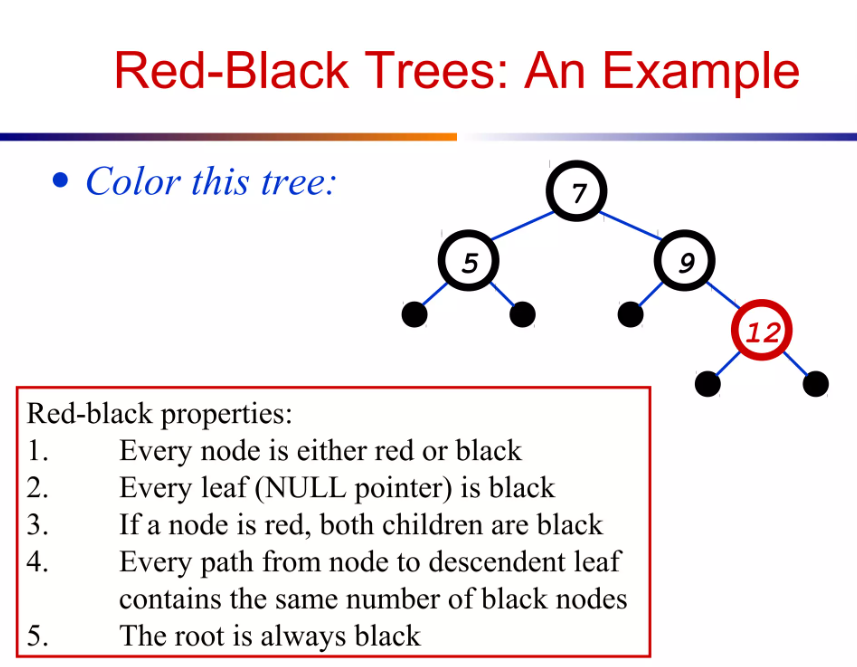
\includegraphics[width=1\textwidth]{img/redblack-example.png}
		\caption{نمونه درخت قرمز-مشکی}
	\end{figure}
	
	
	
	\section{ارتفاع درخت قرمز-سیاه}
	\subsection*{حداکثر ارتفاع}
	\begin{itemize}
		\item حداقل طول درخت \lr{Red-Black} برابر با \textbf{black-height} یا ارتفاع گره‌های مشکی است.
		\item حداقل ارتفاع \lr{h} برای \lr{n} گره برابر است با:
		\[
		h \geq \left\lfloor \log_2(n+1) \right\rfloor
		\]
		این حالت زمانی رخ می‌دهد که درخت \lr{Red-Black} به صورت یک درخت دودویی کامل باشد، یعنی:
		\[
		n = 2^h - 1
		\]
		\item در بدترین حالت، ارتفاع \lr{Red-Black Tree} از رابطه زیر پیروی می‌کند:
		\[
		h \leq 2\log_2(n+1)
		\]
	\end{itemize}
	
	
	% --- بخش جدید اضافه شده ---
	\section{چرخش در درخت قرمز-سیاه}
	چرخش‌ها عملیات اصلی برای حفظ ویژگی‌های درخت قرمز-سیاه در حین درج و حذف هستند. این عملیات به صورت محلی ساختار درخت را تغییر می‌دهند اما خاصیت درخت جستجوی دودویی را حفظ می‌کنند و در زمان \(O(1)\) انجام می‌شوند. دو نوع چرخش وجود دارد: چرخش به چپ و چرخش به راست.
	
	\subsection{LEFT-ROTATE}
	در چرخش به چپ حول گره \(x\)، فرض می‌شود که فرزند راست آن یعنی \(y\) تهی نیست. این چرخش باعث می‌شود \(y\) به جای \(x\) قرار گیرد و \(x\) به عنوان فرزند چپ \(y\) درآید. زیردرخت چپ \(y\) نیز به عنوان زیردرخت راست \(x\) متصل می‌شود.
	
	\begin{figure}[H]
		\centering
		 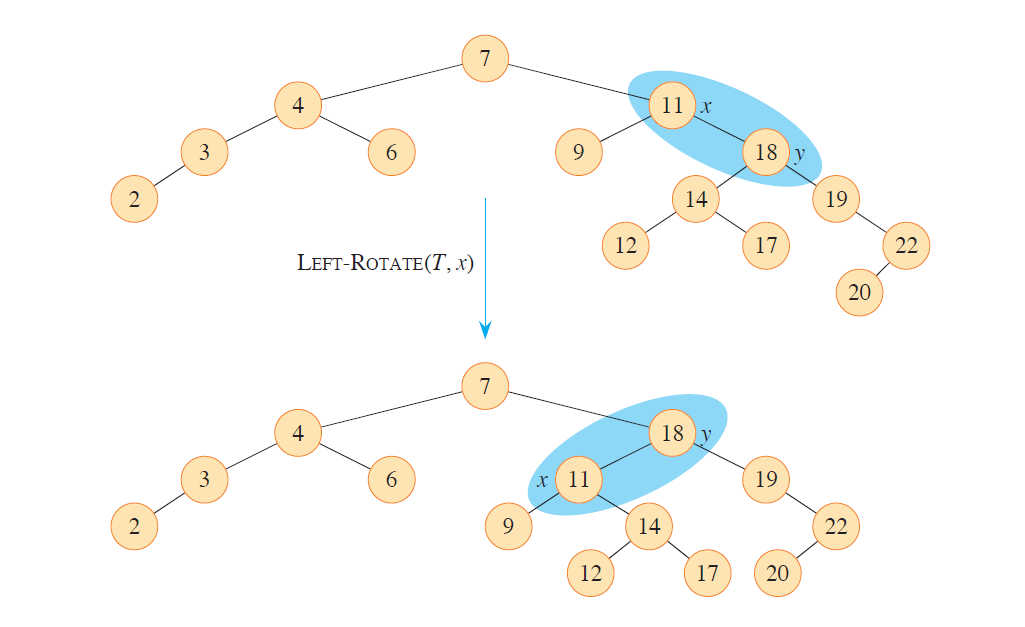
\includegraphics[width=1.2\textwidth]{img/left-rotation.png} % کاربر باید این تصویر را فراهم کند
		\caption{عملکرد چرخش به چپ حول گره x}
	\end{figure}
	
	\begin{LTR}
		\begin{lstlisting}[caption={Left Rotation Pseudocode}, label={lst:left-rotate}]
			LEFT-ROTATE(T, x):
				y = x.right
				x.right = y.left
				if y.left != T.nil:
					y.left.p = x
				y.p = x.p
				if x.p == T.nil:
					T.root = y
				else if x == x.p.left:
					x.p.left = y
				else:
					x.p.right = y
				y.left = x
				x.p = y
		\end{lstlisting}
	\end{LTR}
	
	\subsection{RIGHT-ROTATE}
	چرخش به راست عملیات معکوس چرخش به چپ است. در این چرخش حول گره \( y\)، فرض می‌شود که فرزند چپ آن یعنی \(x\) تهی نیست.
	
	\begin{figure}[H]
		\centering
		 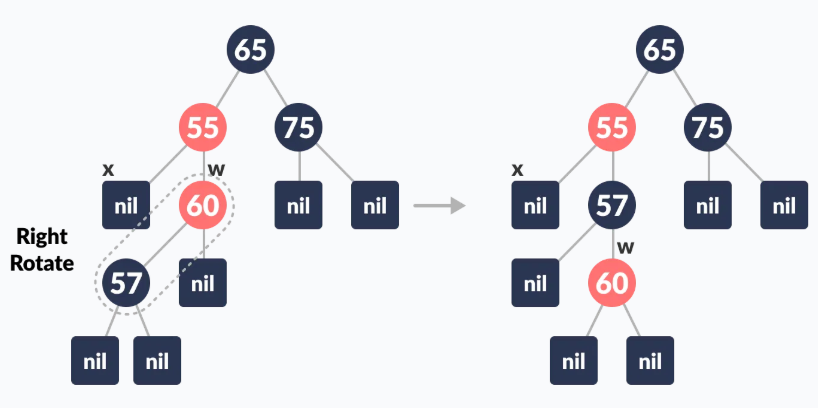
\includegraphics[width=1.1\textwidth]{img/right-rotation.png} % کاربر باید این تصویر را فراهم کند
		\caption{عملکرد چرخش به راست حول گره y=w}
	\end{figure}
	
	\begin{LTR}
		\begin{lstlisting}[caption={Right Rotation Pseudocode}, label={lst:right-rotate}]
			RIGHT-ROTATE(T, y):
				x = y.left
				y.left = x.right
				if x.right != T.nil:
					x.right.p = y
				x.p = y.p
				if y.p == T.nil:
					T.root = x
				else if y == y.p.right:
					y.p.right = x
				else:
					y.p.left = x
				x.right = y
				y.p = x
		\end{lstlisting}
	\end{LTR}
	% --- پایان بخش جدید ---
	
	
	\section{درج در درخت قرمز-سیاه}
	درج گره جدید ممکن است باعث نقض قوانین درخت شود و ساختار آن را به هم بزند. در این شرایط، برای حفظ خاصیت‌های درخت، از چرخش‌ها و رنگ‌آمیزی مجدد استفاده می‌شود. این اصلاحات باعث می‌شوند که درخت به حالت متعادل و درست بازگردد. هدف اصلی این است که خاصیت‌های اساسی درخت مانند تعادل رنگ‌ها و ترتیب گره‌ها حفظ شود. بر اساس وضعیت درخت پس از درج گره، سه حالت مختلف ممکن است پیش بیاید. هر یک از این حالات نیازمند راه‌حل خاص خود است که با چرخش‌ها و تغییر رنگ‌ها اصلاح می‌شود. این فرآیندها به صورت خودکار و مرحله به مرحله انجام می‌گیرند.
	در ادامه، هر یک از این حالت‌ها به صورت دقیق و گام به گام بررسی خواهند شد.
	
	\subsection*{کد الگوریتم درج}
	
	\begin{LTR}
		\begin{lstlisting}[caption={Red-Black Tree Insertion}, label={lst:rb-insert}]
			RB-Insert(T, z):
				y = NIL
				x = T.root
				while x != NIL:
					y = x
					if z.key < x.key:
					x = x.left
					else:
						x = x.right
				z.p = y
				if y == NIL:
					T.root = z
				else if z.key < y.key:
					y.left = z
				else:
					y.right = z
				z.left = NIL
				z.right = NIL
				z.color = RED
				RB-Insert-Fixup(T, z)
		\end{lstlisting}
	\end{LTR}
	
			\subsection*{حالت ۱: عموی گره جدید (y) قرمز است}
		
		
		در این حالت، عموی گره 
		x
		(که تازه درج شده) قرمز رنگ است. این وضعیت ساده‌ترین حالت است و با تغییر رنگ‌های مربوطه حل می‌شود.
		
		\begin{enumerate}
			\item گره والد 
			p
			و عموی 
			y
			گره 
			x
			را به رنگ مشکی در می‌آوریم.
			\item گره پدربزرگ 
			p−>p
			را به رنگ قرمز در می‌آوریم.
			\item اشاره‌گر 
			x
			را به گره پدربزرگ منتقل می‌کنیم تا در تکرار بعدی حلقه (در صورت لزوم) بررسی‌ها از آنجا ادامه پیدا کند.
		\end{enumerate}
		
		این عملیات به گونه‌ای انجام می‌شود که تعداد گره‌های مشکی در مسیرهای مختلف درخت حفظ شود.
		
		\begin{figure}[h!]
			\centering
			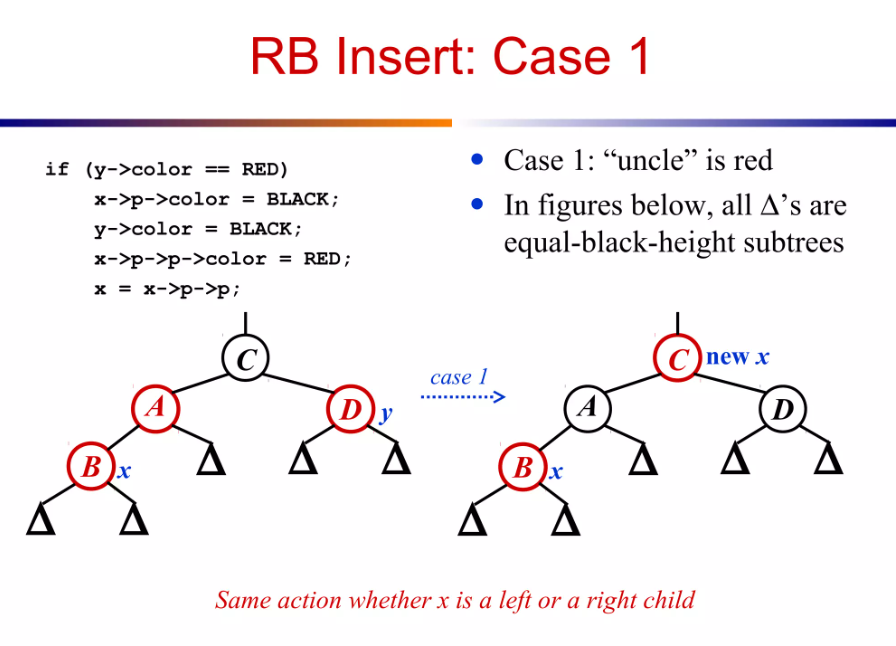
\includegraphics[width=1.1\textwidth]{img/insert-case1.png}
			\caption{درج در درخت قرمز-مشکی: حالت ۱}
		\end{figure}
		
			\subsection*{حالت ۲: عموی گره جدید (y) مشکی است و گره x فرزند راست است}
									
									در این حالت، عموی گره x مشکی رنگ است و گره x یک فرزند راست برای والد خود p است. برای حل این وضعیت، ابتدا باید این حالت را به حالت ۳ تبدیل کنیم.
									
									\begin{enumerate}
										\item یک چرخش به چپ (left rotation) روی گره $x$ انجام می‌دهیم.
										\item پس از چرخش، وضعیت گره‌ها به گونه‌ای می‌شود که می‌توانیم آن را به عنوان حالت ۳ در نظر بگیریم و ادامه عملیات را طبق آن حالت پیش ببریم.
									\end{enumerate}
									
									این تبدیل اطمینان حاصل می‌کند که خاصیت ۴ (تمام مسیرهای پایین‌رونده حاوی تعداد یکسانی از گره‌های مشکی هستند) حفظ شود.
									
									\begin{figure}[H]
										\centering
										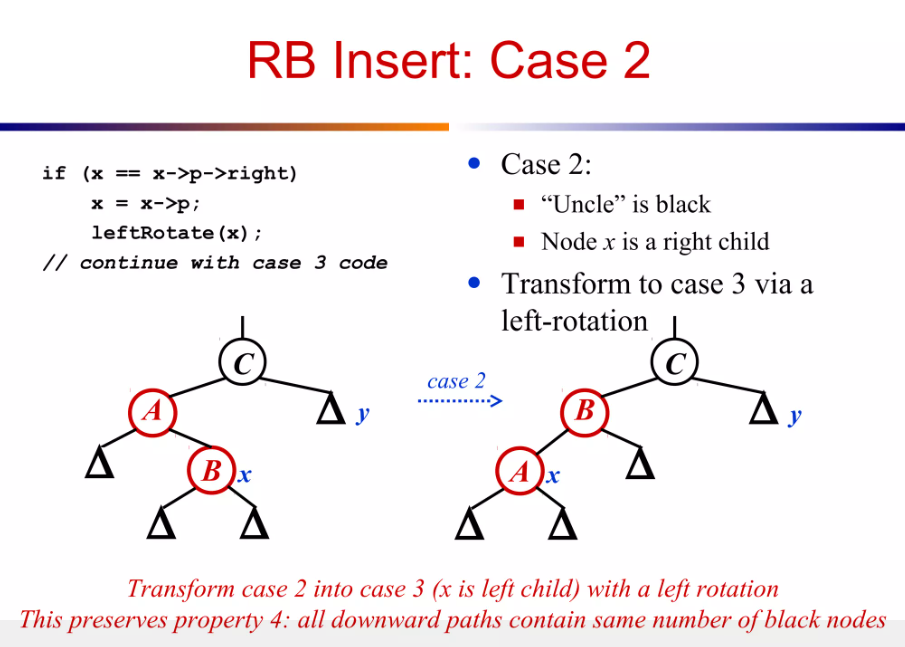
\includegraphics[width=1.1\textwidth]{img/insert-case2.png} % اطمینان حاصل کنید مسیر تصویر صحیح است
										\caption{درج در درخت قرمز-مشکی: حالت ۲}
									\end{figure}
									
									\vspace{10pt}
									
در ادامه حالت سوم را بررسی می کنیم :
			\subsection*{حالت ۳: عموی گره جدید (y) مشکی است و گره x فرزند چپ است}
							
							این حالت معمولاً پس از حالت ۲ (در صورت نیاز به تبدیل) یا به صورت مستقیم رخ می‌دهد. در این وضعیت، عموی گره $x$ مشکی است و گره $x$ یک فرزند چپ برای والد خود $p$ است.
							
							\begin{enumerate}
								\item رنگ گره والد $p$ را به مشکی تغییر می‌دهیم.
								\item رنگ گره پدربزرگ $p->p$ را به قرمز تغییر می‌دهیم.
								\item یک چرخش به راست (right rotation) روی گره پدربزرگ $p->p$ انجام می‌دهیم.
							\end{enumerate}
							
							این عملیات با حفظ خاصیت‌های درخت قرمز-مشکی، تعادل را برقرار می‌کند.
							
							
							
							شکل زیر حالت سوم اضافه کردن گره را نشان می دهد :
							
							
							\begin{figure}[H]
								\centering
								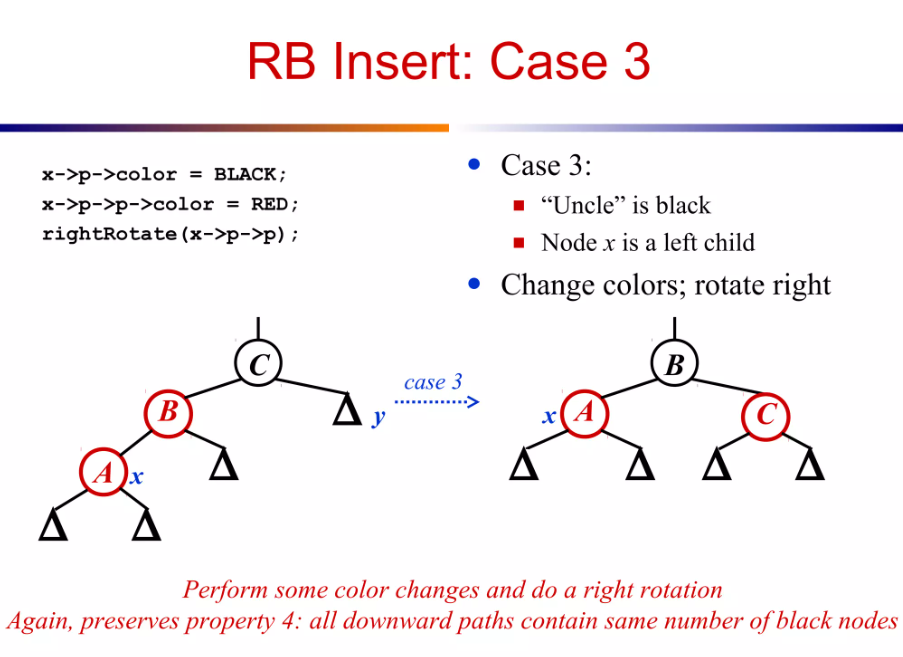
\includegraphics[width=1.1\textwidth]{img/insert-case3.png} % اطمینان حاصل کنید مسیر تصویر صحیح است
								\caption{درج در درخت قرمز-مشکی: حالت ۳}
							\end{figure}
								

	
	
	
	\subsection{FIXUP درج در درخت قرمز-سیاه}
	
	
	در هنگام درج گره، ممکن است خاصیت‌های درخت قرمز-مشکی نقض شود که با اجرای الگوریتم \lr{Fixup}   و اعمال چرخش و رنگ‌آمیزی، تعادل آن بازگردانده می‌شود.

% اضافه کردن الگوریتم RB-Insert-Fixup با همان فرمت
	\begin{LTR}
		\begin{lstlisting}[caption={RB-INSERT-FIXUP}, label={lst:rb-insert-fixup}]
			RB-INSERT-FIXUP(T, z):
				while z.p.color == RED
					if z.p == z.p.p.left // is z's parent a left child?
						y = z.p.p.right // is z's uncle
						if y.color == RED // are z's parent and uncle both red?
							z.p.color = BLACK
							y.color = BLACK
							z.p.p.color = RED
							z = z.p.p // case 1
						else // uncle is black
							if z == z.p.right // case 2
								z = z.p
								LEFT-ROTATE(T, z)
							// case 3
							z.p.color = BLACK
							z.p.p.color = RED
							RIGHT-ROTATE(T, z.p.p)
					else // same as lines 3-15, but with "right" and "left" exchanged
						y = z.p.p.left
						if y.color == RED
							z.p.color = BLACK
							y.color = BLACK
							z.p.p.color = RED
							z = z.p.p
						else
							if z == z.p.left
								z = z.p
								RIGHT-ROTATE(T, z)
							z.p.color = BLACK
							z.p.p.color = RED
							LEFT-ROTATE(T, z.p.p)
				T.root.color = BLACK
		\end{lstlisting}
	\end{LTR}

	\begin{figure}[H]
	\centering
	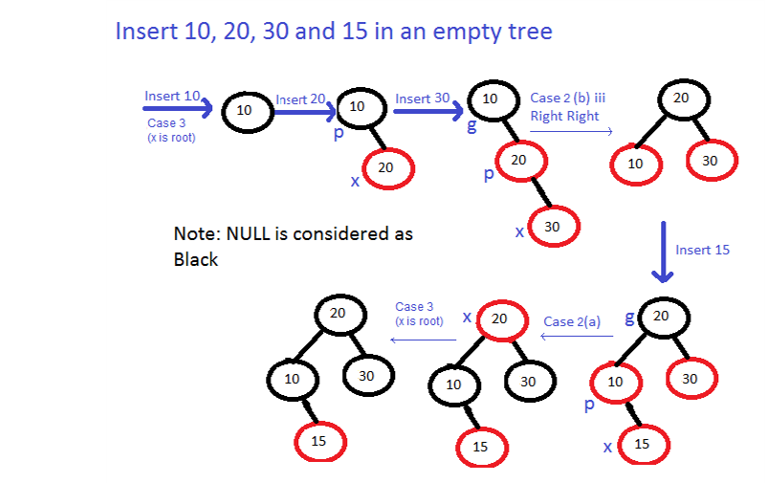
\includegraphics[width=0.9\textwidth]{img/insert-fixup.png} % اطمینان حاصل کنید مسیر تصویر صحیح است
	\caption{مثال اجرای \lr{Fixup}   بعد از هر بار \lr{insert}   کردن}
	
	\end{figure}
		\begin{figure}[H]
		\centering
		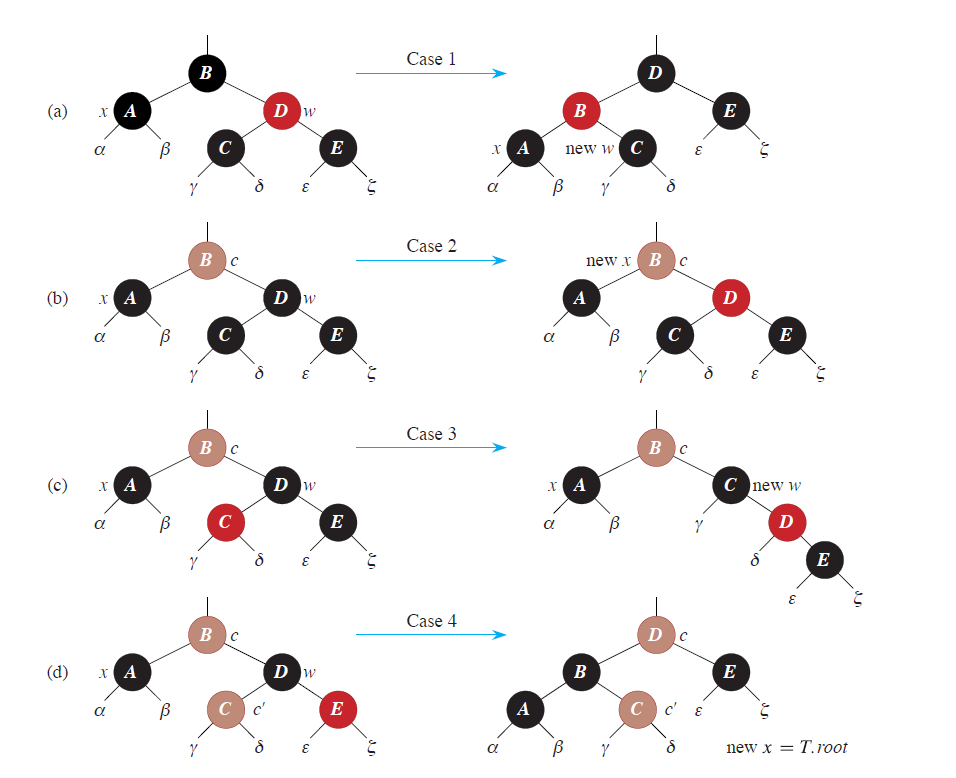
\includegraphics[width=0.9\textwidth]{img/insert-fixup2.png} % اطمینان حاصل کنید مسیر تصویر صحیح است
		\caption{مثال اجرای \lr{Fixup}   بعد از هر بار \lr{insert}   کردن}
	\end{figure}
	
	
	\section{حذف در درخت قرمز-سیاه}

	
حذف در درخت قرمز-مشکی پیچیده‌تر از درج است، زیرا ممکن است تعادل گره‌های مشکی یا قوانین رنگ نقض شود.
الگوریتم\lr{RB-DELETE}گره را با جانشین مناسب جایگزین کرده و در صورت نیاز، با اجرای \lr{RB-DELETE-FIXUP} توازن درخت را بازمی‌گرداند.
در ادامه، این الگوریتم را بررسی می‌کنیم.
	
	\begin{LTR}
		\begin{lstlisting}[caption={Red-Black Tree Deletion}, label={lst:rb-delete}]
			RB-DELETE(T, z)
				y = z
				y-original-color = y.color
				if z.left == T.nil
					x = z.right
					RB-TRANSPLANT(T, z, z.right)              // replace z by its right child
				elseif z.right == T.nil
				x = z.left
				RB-TRANSPLANT(T, z, z.left)               // replace z by its left child
				else
					y = TREE-MINIMUM(z.right)                 // y is z's successor
					y-original-color = y.color
					x = y.right
					if y ≠ z.right
						RB-TRANSPLANT(T, y, y.right)          // replace y by its right child
						y.right = z.right
						y.right.p = y
					else
						x.p = y                                // in case x is T.nil
					RB-TRANSPLANT(T, z, y)                    // replace z by y
					y.left = z.left                           // and give z's left child to y
					y.left.p = y
					y.color = z.color
				if y-original-color == BLACK
					RB-DELETE-FIXUP(T, x)                     // correct any violations
			
		\end{lstlisting}
	\end{LTR}
	
		\subsection{RB-DELETE-FIXUP }
		

			پس از حذف یک گره در درخت قرمز-مشکی، اگر گره حذف‌شده یا جانشین آن مشکی باشد، ممکن است قوانین قرمز-مشکی نقض شوند. \\
			الگوریتم \texttt{RB-DELETE-FIXUP} برای بازگرداندن این خاصیت‌ها اجرا می‌شود. \\
			این الگوریتم با پیمایش از گره \texttt{x} به سمت ریشه، با چرخش‌ها و تغییر رنگ‌ها تعادل درخت را بازمی‌گرداند.

		
			\begin{LTR}
				\begin{lstlisting}[caption={Red-Black Tree Deletion}, label={lst:rb-delete}]
					RB-DELETE-FIXUP(T, x)
						while x ≠ T.root and x.color = BLACK
						if x = x.p.left //case1
							w = x.p.right
							if w.color = RED
								w.color = BLACK
								x.p.color = RED
								LEFT-ROTATE(T, x.p)
								w = x.p.right
							if w.left.color = BLACK and w.right.color = BLACK  //case2
								w.color = RED
								x = x.p
							else
								if w.right.color = BLACK //case3
									w.left.color = BLACK
									w.color = RED
									RIGHT-ROTATE(T, w)
									w = x.p.right
								w.color = x.p.color // case4
								x.p.color = BLACK
								w.right.color = BLACK
								LEFT-ROTATE(T, x.p)
								x = T.root
						else 
							(*@ // same as then-clause with "right" and "left" exchanged @*)

				\end{lstlisting}
			\end{LTR}
			
			
	\vspace{20pt}
	
	\begin{figure}[H]
		\centering
		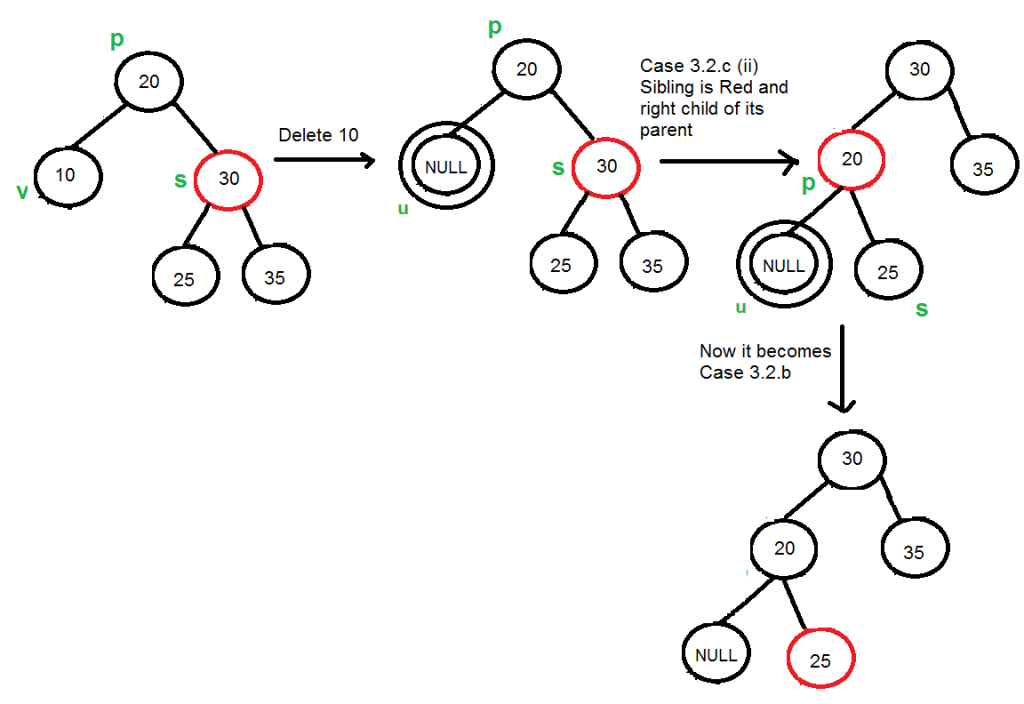
\includegraphics[width=1.0\textwidth]{img/delete-fixup.png} % اطمینان حاصل کنید مسیر تصویر صحیح است
		\caption{مثال اجرای \lr{Fixup}   بعد از هر بار \lr{Delete}   کردن}
	\end{figure}
	
	
			\subsection{RB-DELETE-FIXUP مثال پیشرفته }
			در ادامه یک مثال پیشرفته و چند مرحله ای از حذف گره را تا زمان برقراری کامل تعادل بررسی می کنیم :
	\begin{figure}[H]
		\centering
		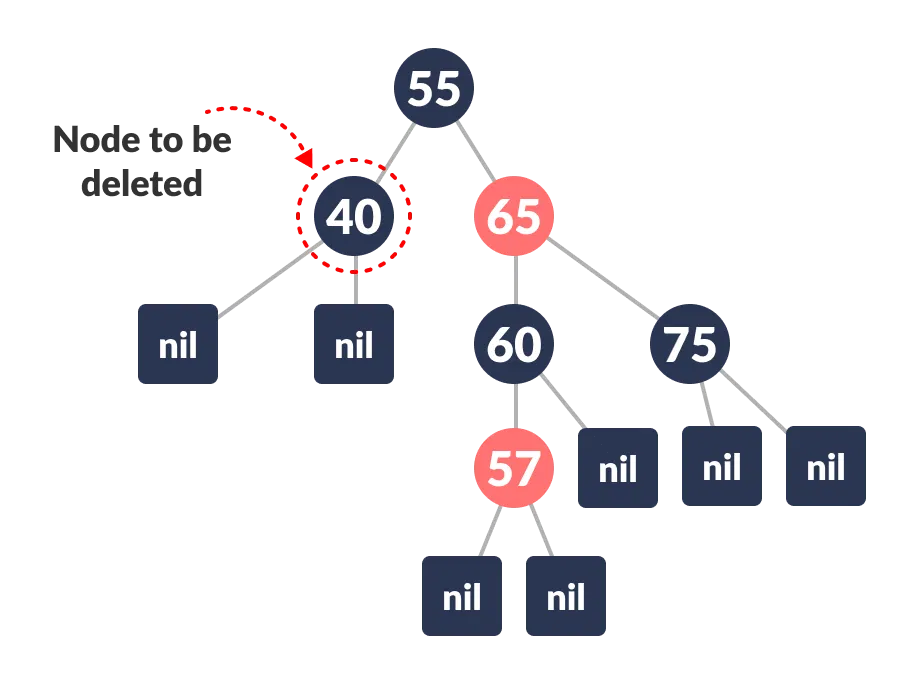
\includegraphics[width=0.5\textwidth]{img/advancedDelFix/delete-1-red-black.png} % اطمینان حاصل کنید مسیر تصویر صحیح است
		\caption{شناسایی گره 40 برای حذف؛ گره 40 یک گره قرمز بدون فرزند است که به سادگی حذف می‌شود.}
	\end{figure}
	
	\begin{figure}[H]
		\centering
		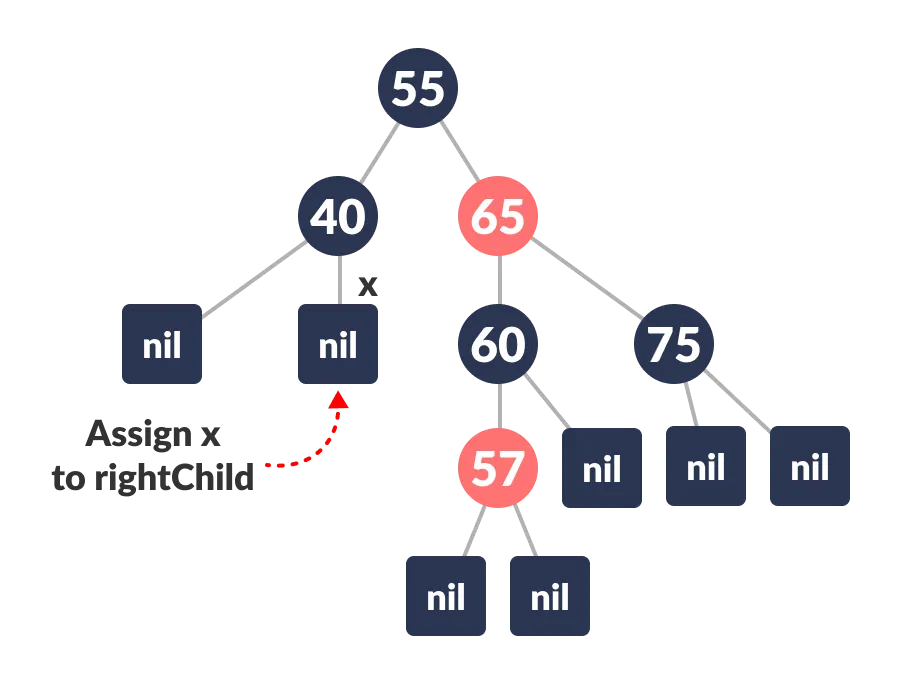
\includegraphics[width=0.7\textwidth]{img/advancedDelFix/delete-2-red-black.png} % اطمینان حاصل کنید مسیر تصویر صحیح است
		\caption{برای حذف 40 ابتدا x را به فرزند راست آن نسبت می‌دهیم.}
	\end{figure}
	
	\begin{figure}[H]
		\centering
		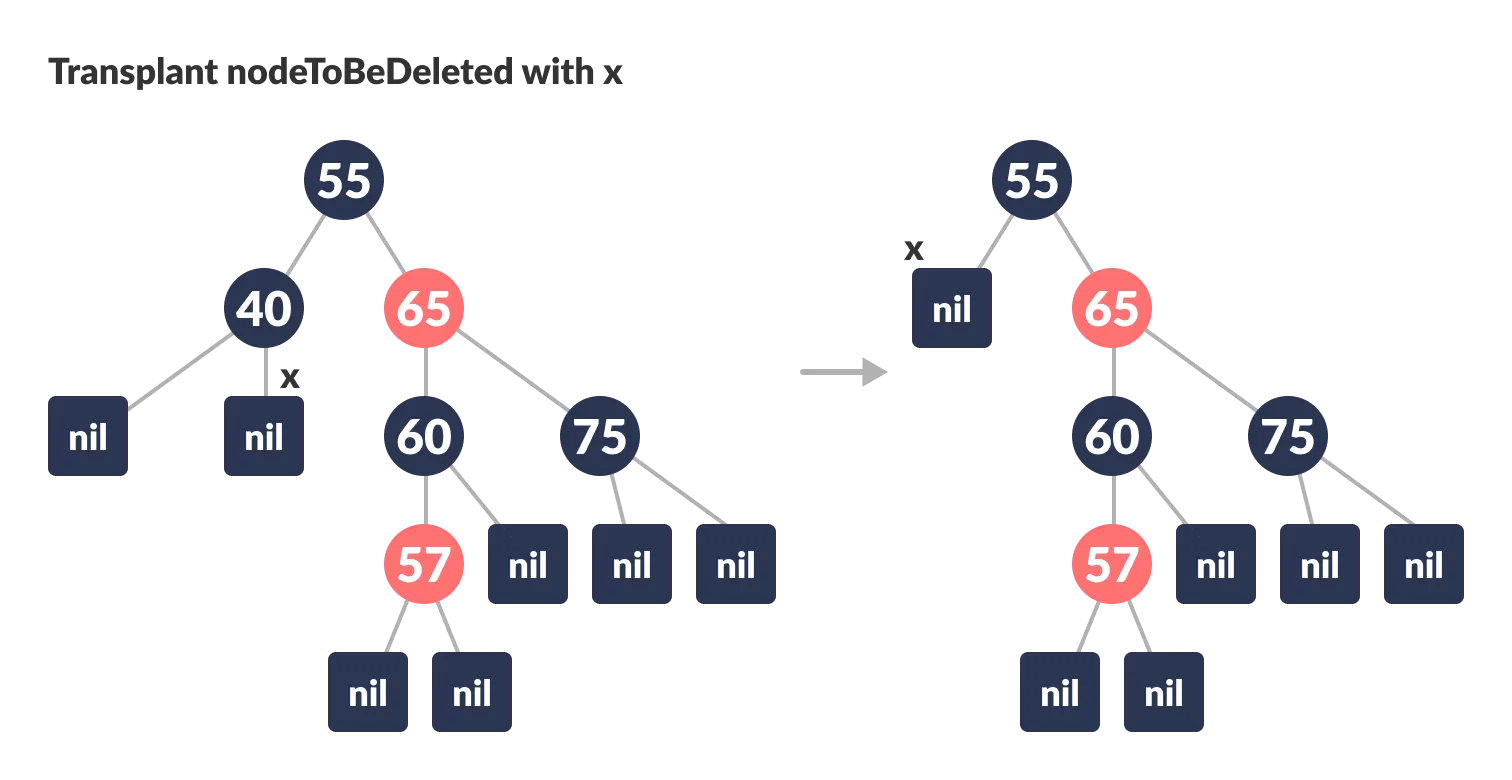
\includegraphics[width=0.7\textwidth]{img/advancedDelFix/delete-3-red-black.png} % اطمینان حاصل کنید مسیر تصویر صحیح است
		\caption{پس از حذف 40، تعداد گره‌های مشکی در مسیرها نابرابر می‌شوند و باید fixup انجام دهیم.}
	\end{figure}
	
	\begin{figure}[H]
		\centering
		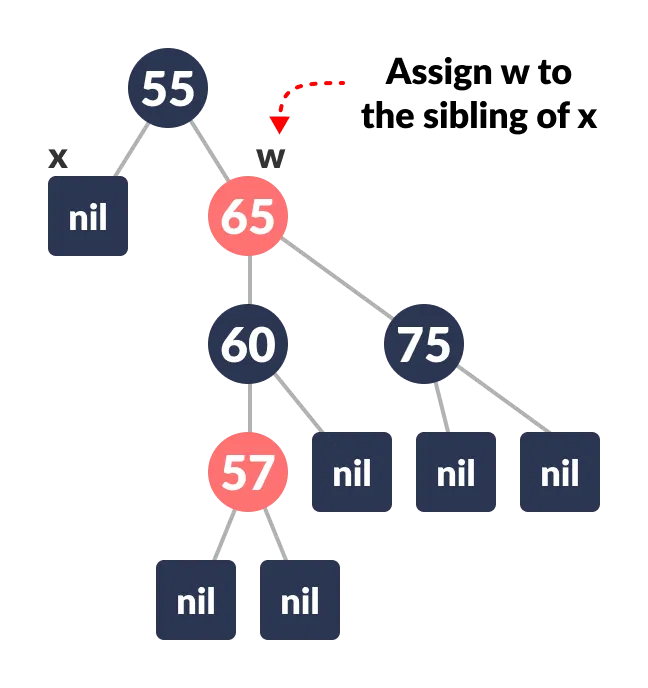
\includegraphics[width=0.5\textwidth]{img/advancedDelFix/delete-4-red-black.png} % اطمینان حاصل کنید مسیر تصویر صحیح است
		\caption{w را به 65 نسبت داده و به عنوان گره برادر/خواهر انتخاب می‌کنیم.}
	\end{figure}
	
	\begin{figure}[H]
		\centering
		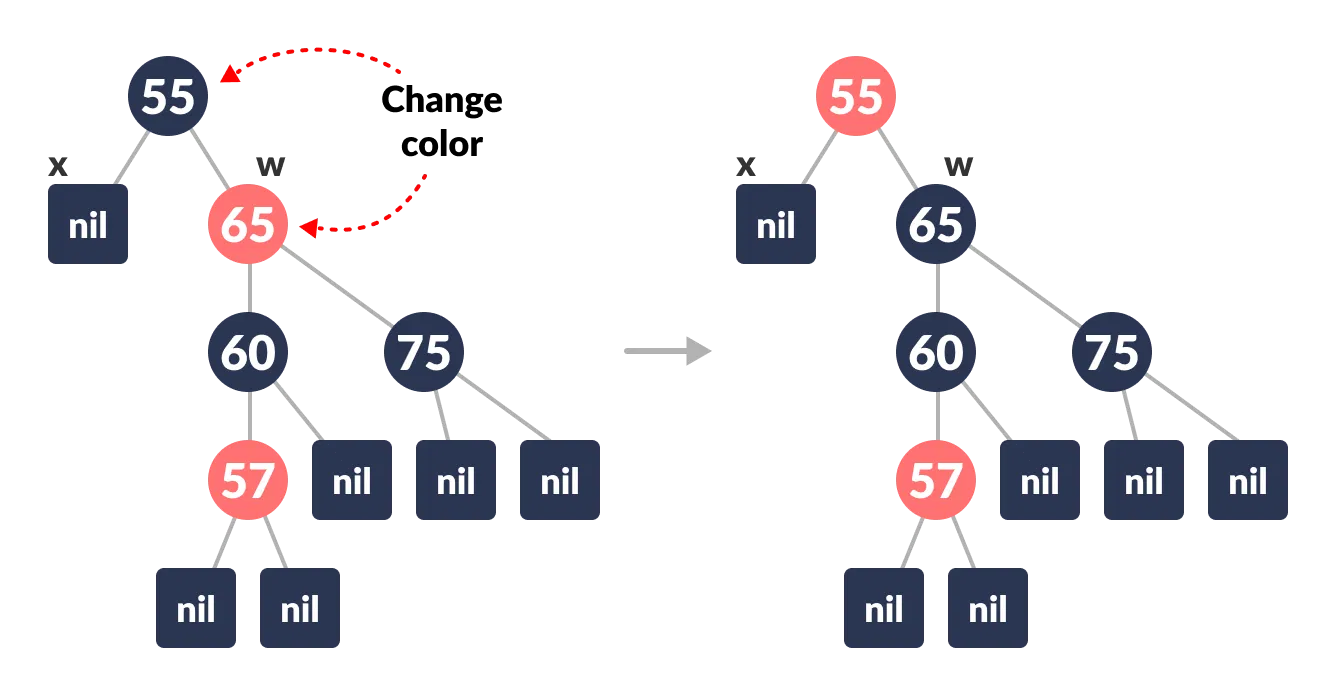
\includegraphics[width=0.5\textwidth]{img/advancedDelFix/delete-5-red-black.png} % اطمینان حاصل کنید مسیر تصویر صحیح است
		\caption{طبق الگوی fixup رنگ 65 و 55 را عوض می‌کنیم.}
	\end{figure}
	
	\begin{figure}[H]
		\centering
		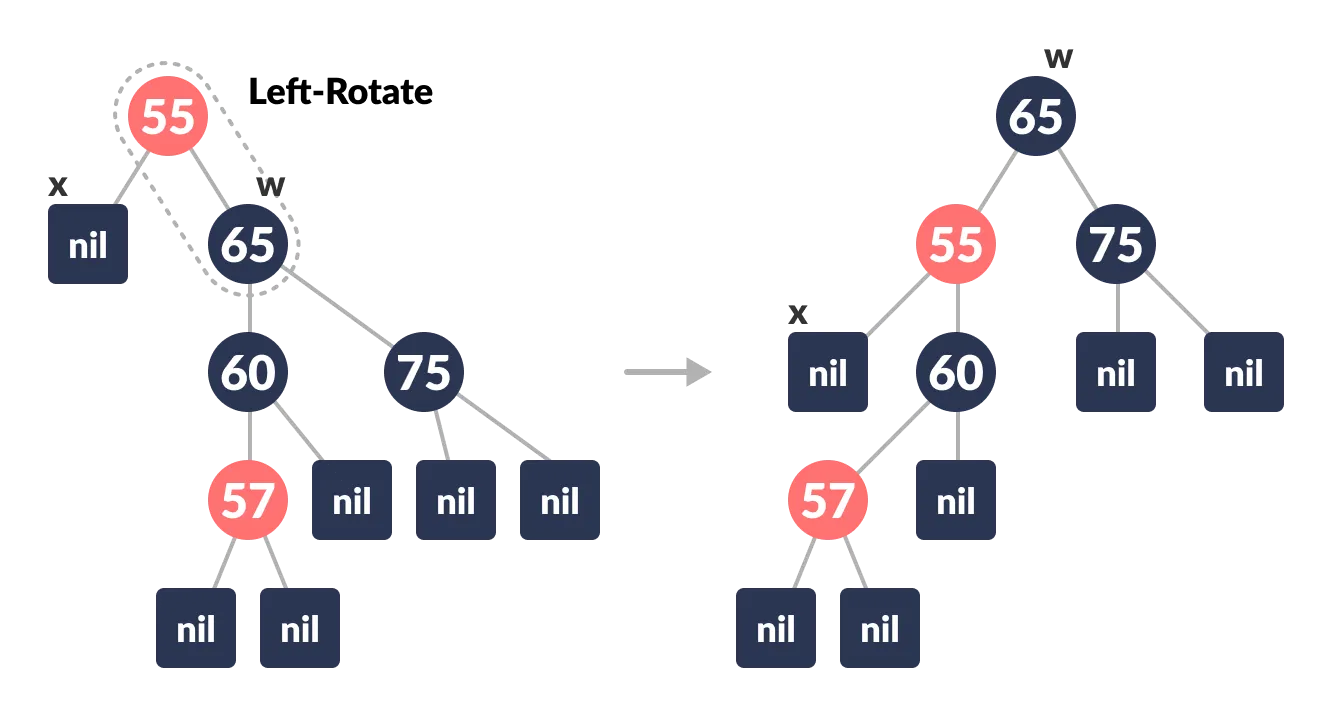
\includegraphics[width=0.5\textwidth]{img/advancedDelFix/delete-6-red-black.png} % اطمینان حاصل کنید مسیر تصویر صحیح است
		\caption{سپس چرخش به چپ حول گره 55 انجام می‌دهیم.}
	\end{figure}
	
	\begin{figure}[H]
		\centering
		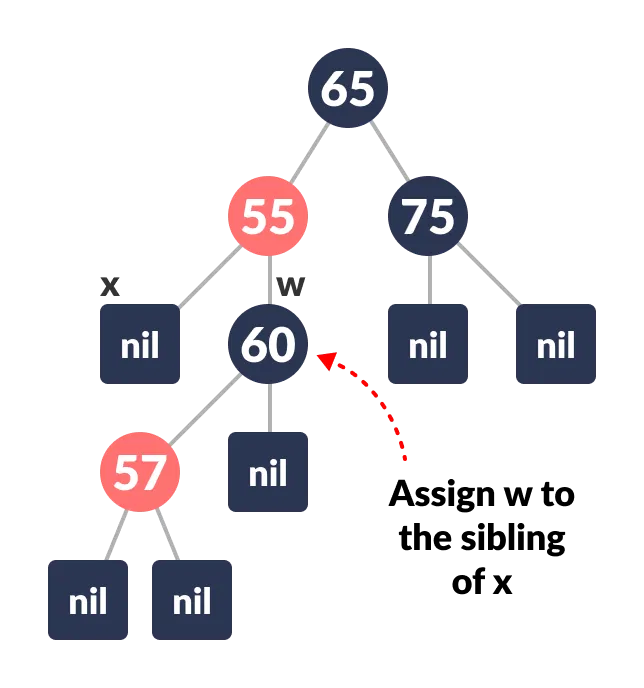
\includegraphics[width=0.5\textwidth]{img/advancedDelFix/delete-7-red-black.png} % اطمینان حاصل کنید مسیر تصویر صحیح است
		\caption{موقعیت فعلی درخت پس از حذف و تعویض. گره 60 به عنوان "w" (برادر) و 'nil' به عنوان "x" (گره دارای دو سیاهی اضافی) مشخص شده است.}
	\end{figure}
	
	\begin{figure}[H]
		\centering
		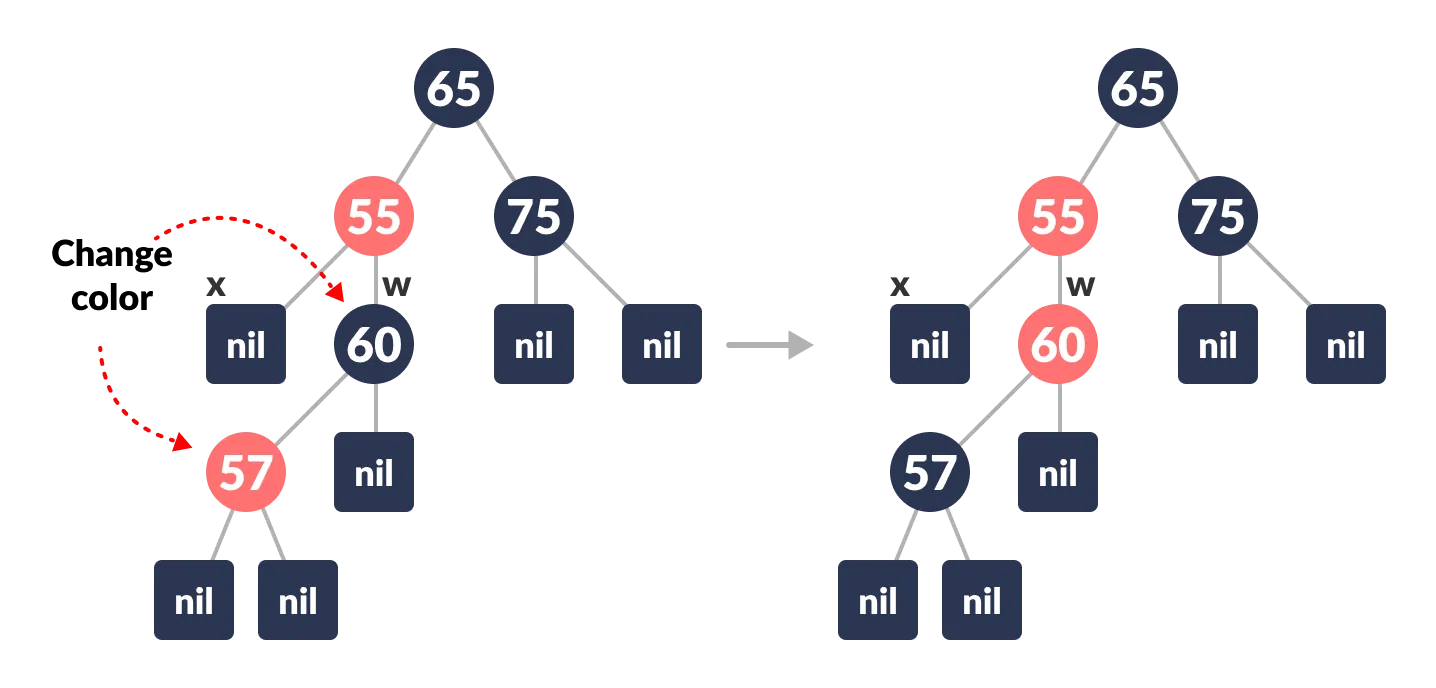
\includegraphics[width=0.5\textwidth]{img/advancedDelFix/delete-8-red-black.png} % اطمینان حاصل کنید مسیر تصویر صحیح است
		\caption{گره 57 از فرزند چپ 60 به فرزند راست 60 منتقل می‌شود و گره 60 رنگ قرمز می‌گیرد.}
	\end{figure}
	
	\begin{figure}[H]
		\centering
		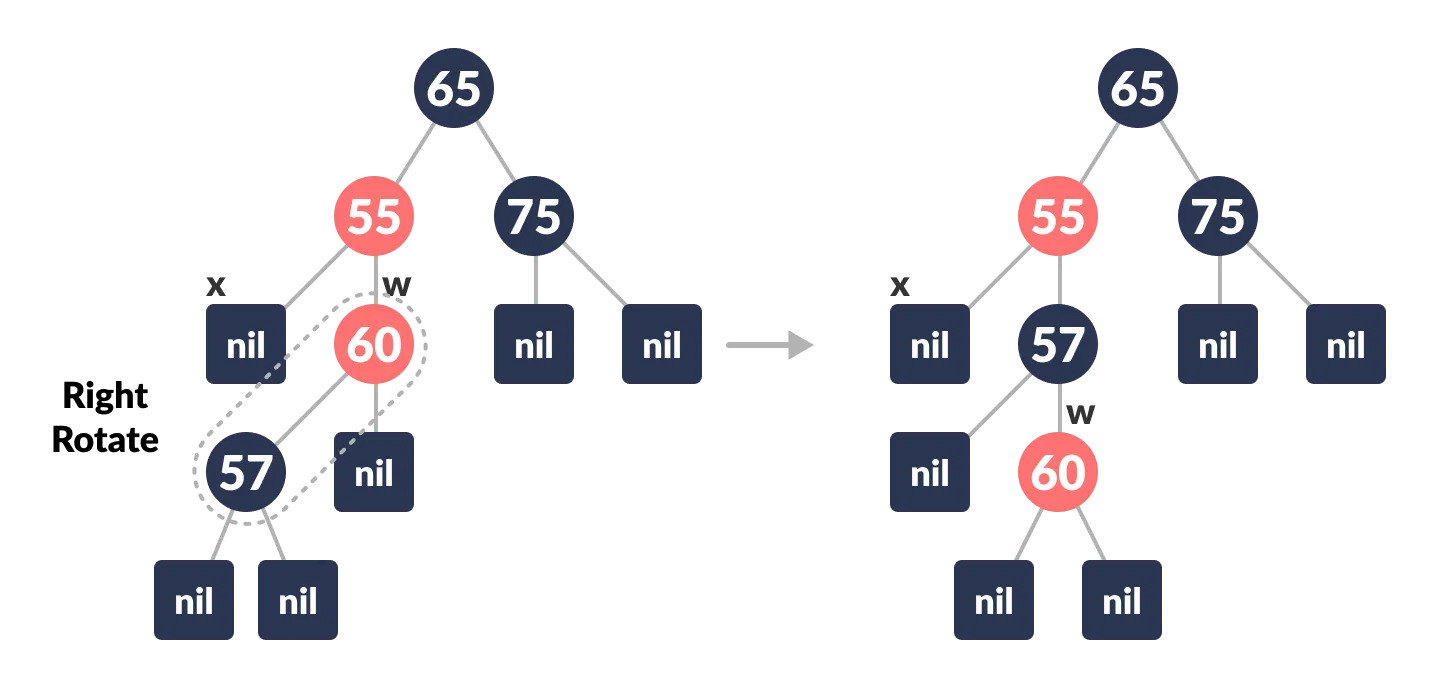
\includegraphics[width=0.5\textwidth]{img/advancedDelFix/delete-9-red-black.png} % اطمینان حاصل کنید مسیر تصویر صحیح است
		\caption{گره 57 جای گره 60 را می‌گیرد و گره 60 به عنوان فرزند راست 57 قرار می‌گیرد. این مرحله شامل تغییر رنگ‌ها برای حفظ خواص قرمز-سیاه است.}
	\end{figure}
	
	\begin{figure}[H]
		\centering
		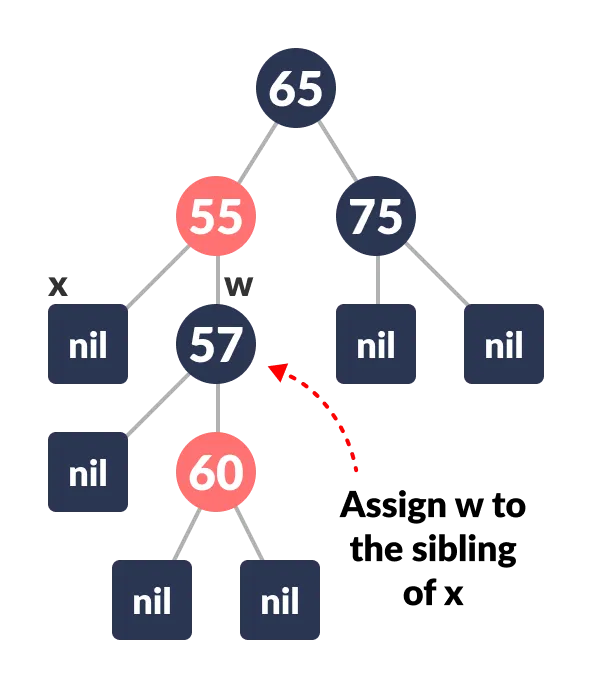
\includegraphics[width=0.5\textwidth]{img/advancedDelFix/delete-10-red-black.png} % اطمینان حاصل کنید مسیر تصویر صحیح است
		\caption{وضعیت پس از حذف گره، که گره 60 به عنوان "x" (نقص دو سیاهی) و گره 57 به عنوان برادر قرمز آن ("sibling") مشخص شده است. (تکرار گام 7، ولی از زاویه دید x)}
	\end{figure}
	
	\begin{figure}[H]
		\centering
		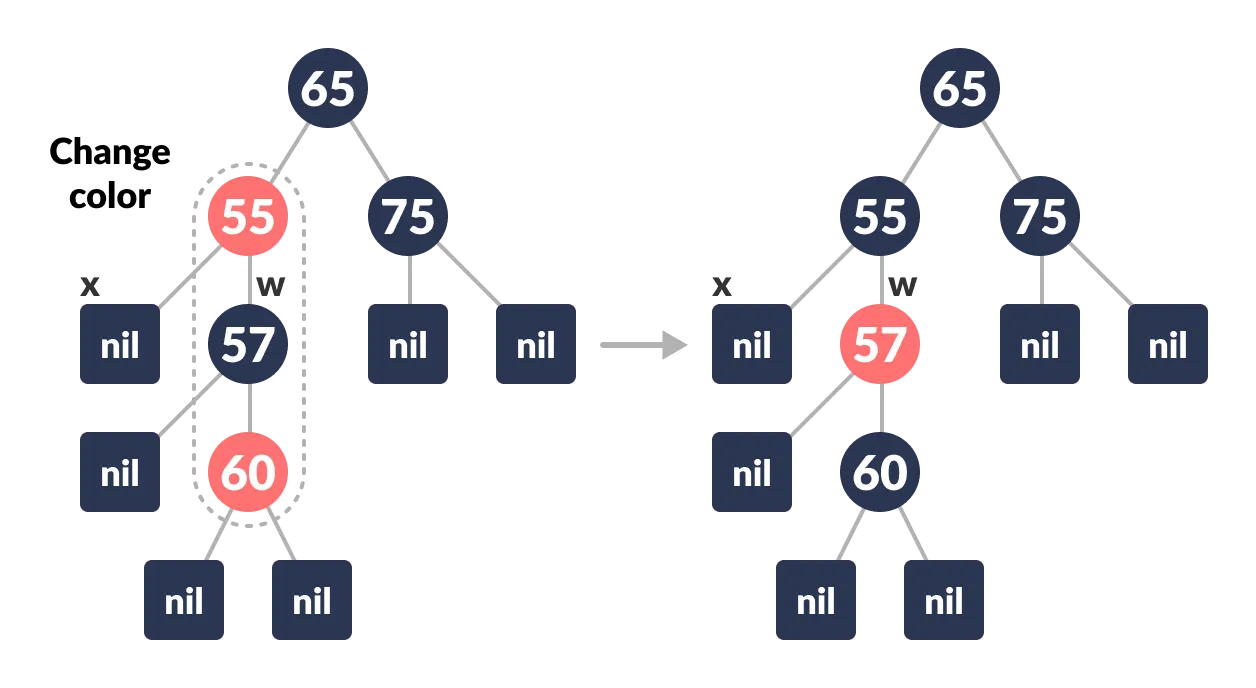
\includegraphics[width=0.5\textwidth]{img/advancedDelFix/delete-11-red-black.png} % اطمینان حاصل کنید مسیر تصویر صحیح است
		\caption{چرخش راست در گره 55 انجام می‌شود تا گره 57 به سمت بالا حرکت کند و رنگ‌ها تنظیم شوند.}
	\end{figure}
	
	\begin{figure}[H]
		\centering
		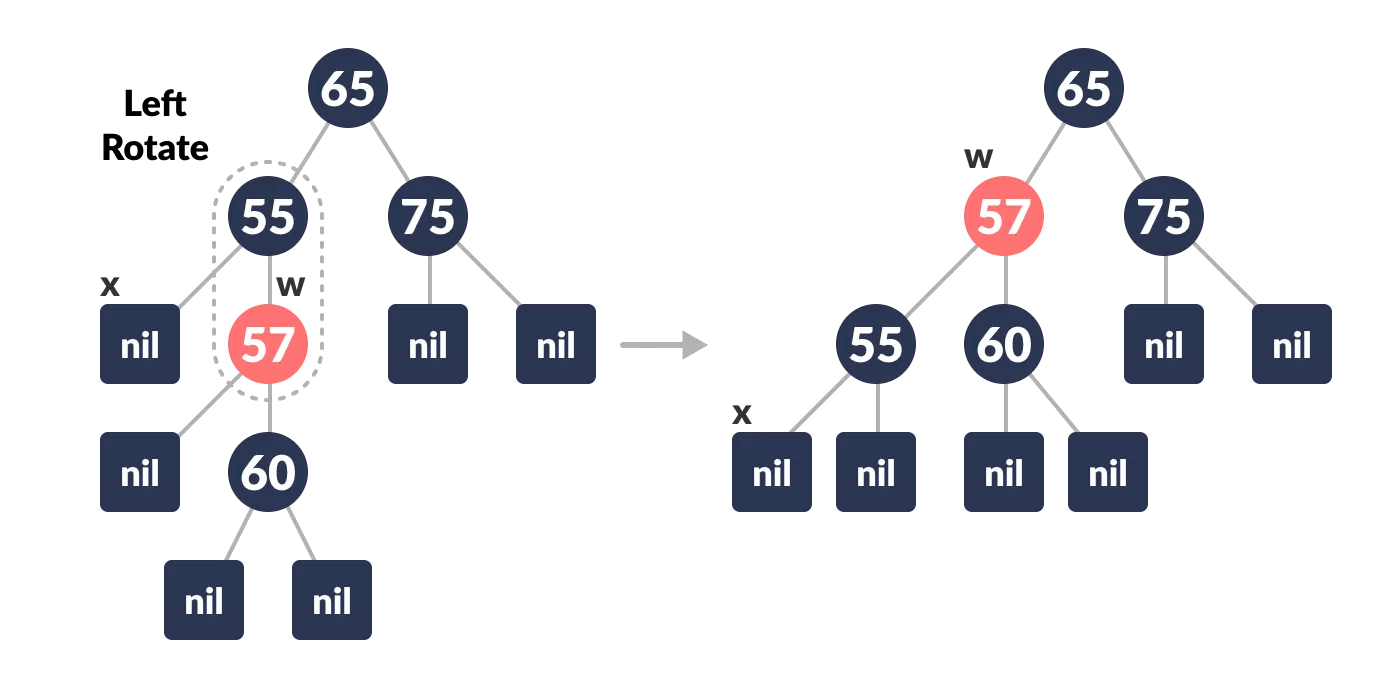
\includegraphics[width=0.5\textwidth]{img/advancedDelFix/delete-12-red-black.png} % اطمینان حاصل کنید مسیر تصویر صحیح است
		\caption{پس از چرخش و تنظیم رنگ‌ها، گره 57 اکنون ریشه زیردرخت شده است و خواص درخت قرمز-سیاه بازسازی شده‌اند.}
	\end{figure}
	
	\begin{figure}[H]
		\centering
		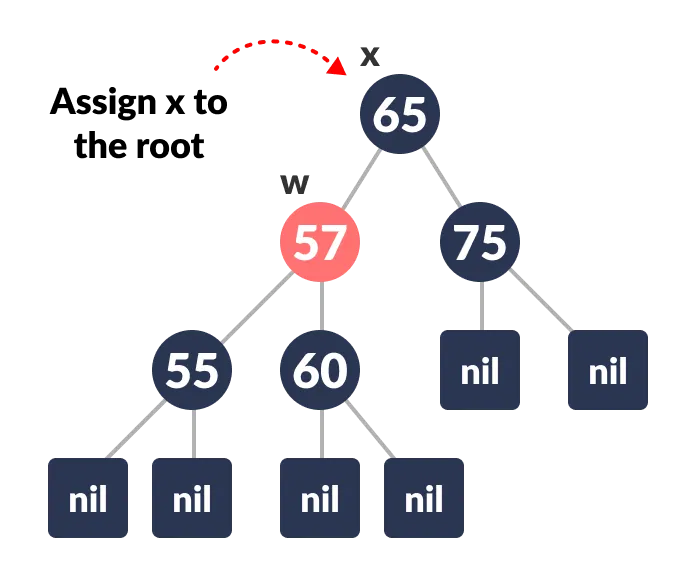
\includegraphics[width=0.5\textwidth]{img/advancedDelFix/delete-13-red-black.png} % اطمینان حاصل کنید مسیر تصویر صحیح است
		\caption{شکل نهایی درخت.}
	\end{figure}

	
	\section{منابع}
	\begin{itemize}
		\item CLRS (ویرایش چهارم)
		\item \lr{https://www.programiz.com/dsa/deletion-from-a-red-black-tree}
		\item \lr{https://medium.com/analytics-vidhya/deletion-in-red-black-rb-tree-92301e1474ea}
		\item \lr{https://www.cs.csubak.edu/~msarr/visualizations/RedBlack.html}
	\end{itemize}
	
\end{document}